\section{Микрораспределение}	
	\subsection{Пала-губа}
Описание микрораспределения макробентоса проводили при помощи метода пространственных автокорреляций с использованием индекса Морана (\cite{Thrush_et_al_1989}).
На литорали Пала-губы достоверные пятна агрегации были обнаружены для {\it Macoma balthica}, {\it Cerastoderma edule} и {\it Priapulus caudatus}. 

Особи {\it M.~balthica} формируют скопления размером около $2-4$~м (рис.~\ref{ris:moransI_Pala_Macoma}). 
Наличие серии достоверно отрицательных значений индекса автокорреляции Морана для больших расстояний свидетельствует о наличии либо градиентого изменения численности, либо крупной агрегации с нечеткими краями.
Наличие градиентного изменения обилия в направлении к руслу ручья было показано с использованием коэффициента корреляции Кендалла ($\tau = 0,55; p = 3,48 \times 10^{-6}$).
Распределение маком по биомассе соответствует распределению по численности. Также корреляционный анализ Кендалла показал градиентное уменьшение биомассы в направлении от моря ($\tau = -0,4; p = 0,0005$).


	\begin{figure}[h]

	\begin{minipage}[b]{.5\linewidth}
	%Фигурка в первом ряду слева размер отведенный под весь этот объект -- 0.46 от ширины строки
	%Параметр [b] означает, что выравнивание этих министраниц будет по нижнему краю
	\begin{center}
	{\small N}
		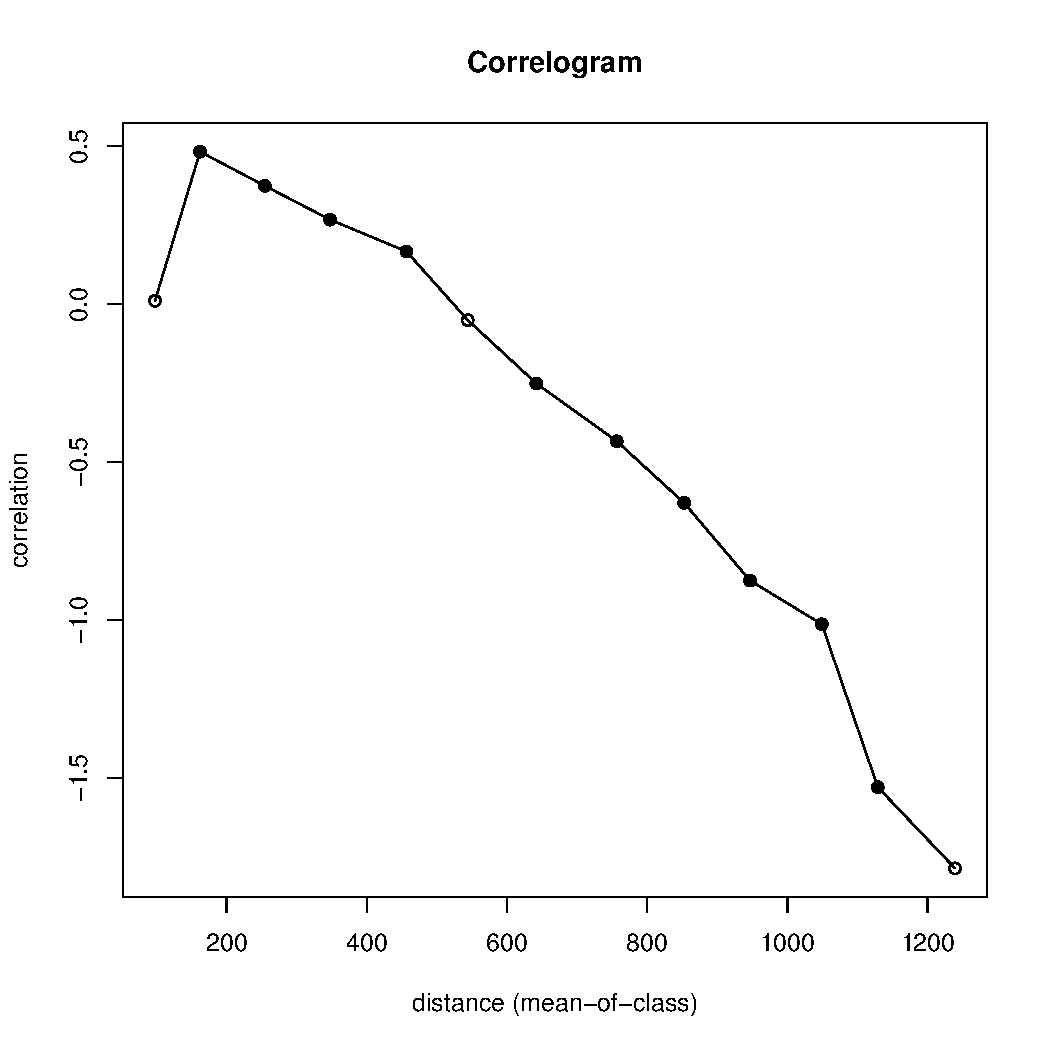
\includegraphics[width=80mm]{../Barenc_Sea/distribution_Moran/Pala_moran_N_Macoma_balthica_.pdf}
	\end{center}
	\end{minipage}
	%
	\hfil %Это пружинка отодвигающая рисунки друг от друга
	%
	\begin{minipage}[b]{.5\linewidth}
	%Следующий рисунок - первый ряд справа %DUNGEON S_4 \ AB
	\begin{center}
	{\small B}
		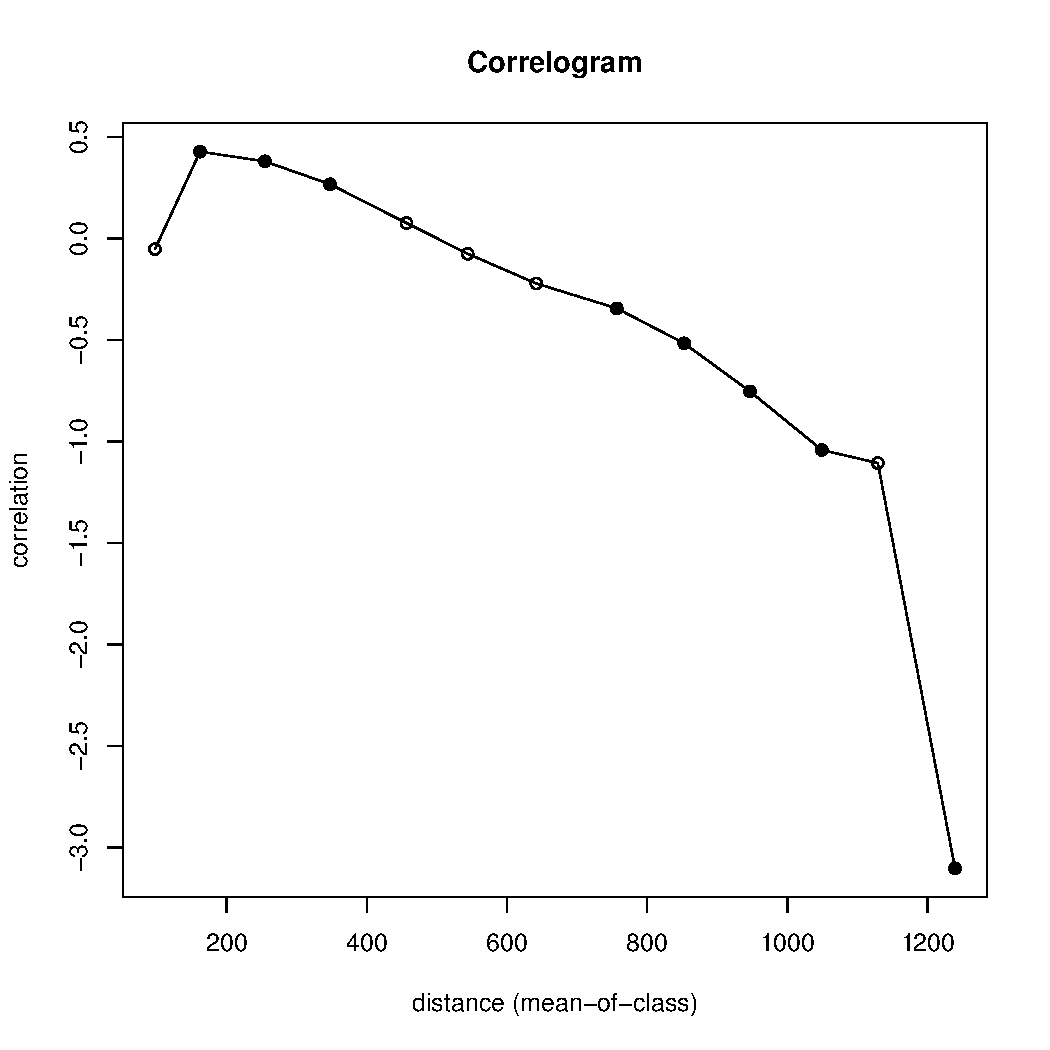
\includegraphics[width=80mm]{../Barenc_Sea/distribution_Moran/Pala_moran_B_Macoma_balthica_.pdf}
	\end{center}
	\end{minipage}
	\caption{Микрораспределение {\it Macoma balthica} на литорали Пала-губы}
	\label{ris:moransI_Pala_Macoma}
	\end{figure}

\textcolor{red}{С {\it C.~edule} непонятно что (рис.~\ref{ris:moransI_Pala_Cerastoderma}). По биомассе - агрегация около 4 м. А численность - при тех же 4 м - отрицательная автокорреляция. Я было решила что это значит что они сидят по штуке на расстоянии 4м? но кажется это фигня. И такие же картинки для Макомы, Церастодермы и Гаммаруса в Дальнезеленецкой (рис.~\ref{ris:moransI_DZ}).}

	\begin{figure}[h]
	\begin{minipage}[b]{.5\linewidth}
	%Фигурка в первом ряду слева размер отведенный под весь этот объект -- 0.46 от ширины строки
	%Параметр [b] означает, что выравнивание этих министраниц будет по нижнему краю
	\begin{center}
	{\small N}
		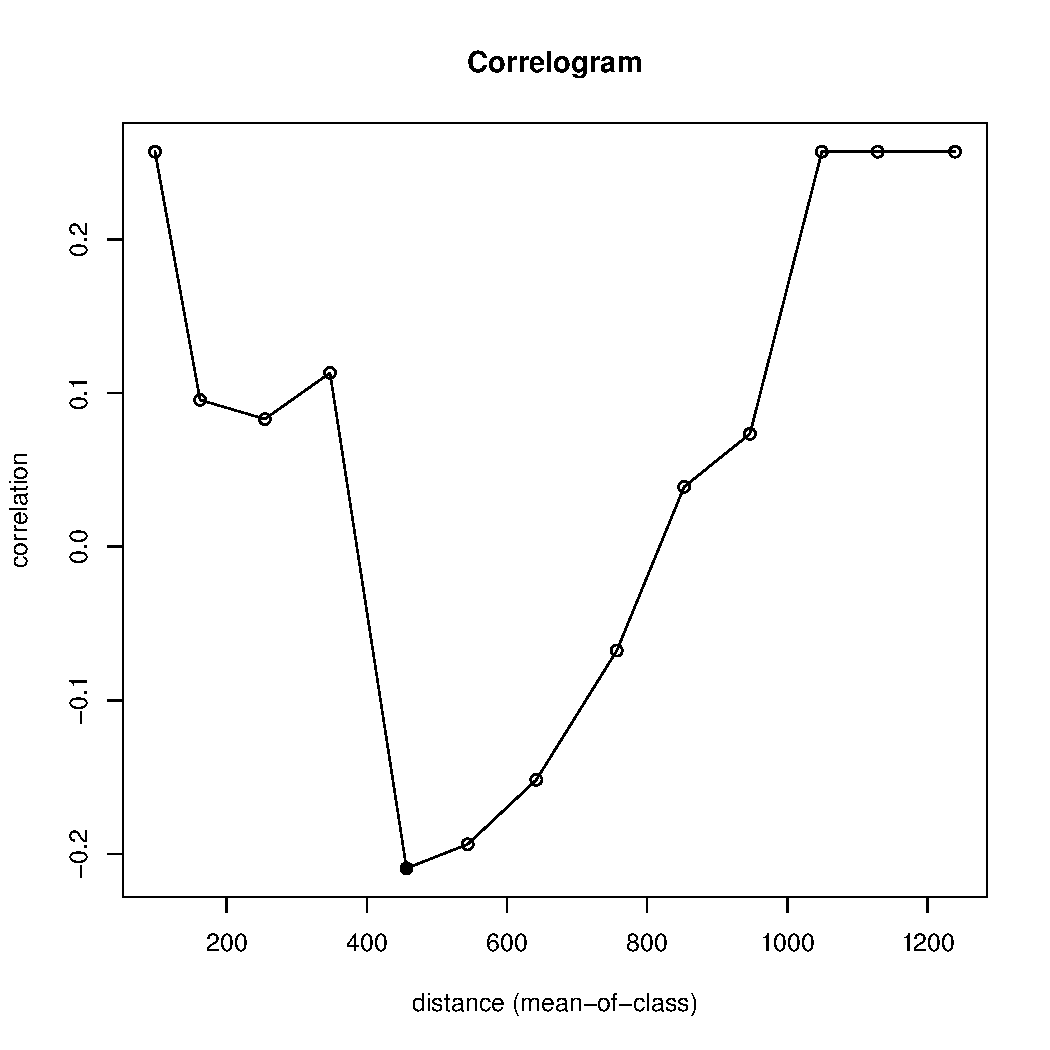
\includegraphics[width=80mm]{../Barenc_Sea/distribution_Moran/Pala_moran_N_Cerastoderma_edule_.pdf}
	\end{center}
	\end{minipage}

	\caption{Микрораспределение {\it Cerastoderma edule} на литорали Пала-губы}
	\label{ris:moransI_Pala_Cerastoderma}
	\end{figure}



	\begin{figure}[h]

	\begin{minipage}[b]{.46\linewidth}
%Фигурка в первом ряду слева размер отведенный под весь этот объект -- 0.46 от ширины строки
%Параметр [b] означает, что выравнивание этих министраниц будет по нижнему краю
	\begin{center}
	{\small N~{\it Macoma balthica} Квадарт 1, 2008}
		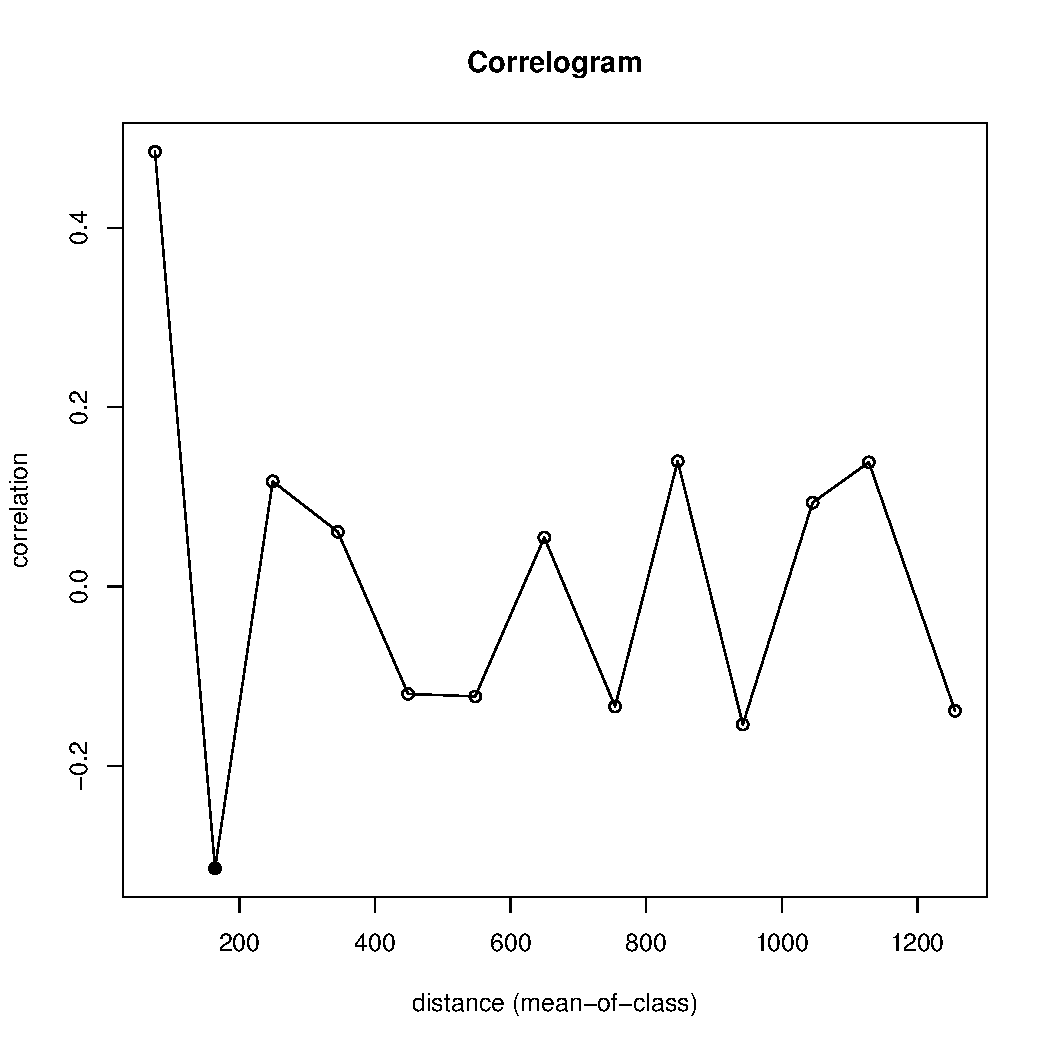
\includegraphics[width=65mm]{../Barenc_Sea/distribution_Moran/Plyazh081_moran_N_Macoma_balthica_.pdf}
	\end{center}
	\end{minipage}
%
	\hfil %Это пружинка отодвигающая рисунки друг от друга
%
	\begin{minipage}[b]{.46\linewidth}
%Следующий рисунок - первый ряд справа %DUNGEON S_4 \ AB
	\begin{center}
	{\small B~{\it Macoma balthica} Квадарт 1, 2008}
		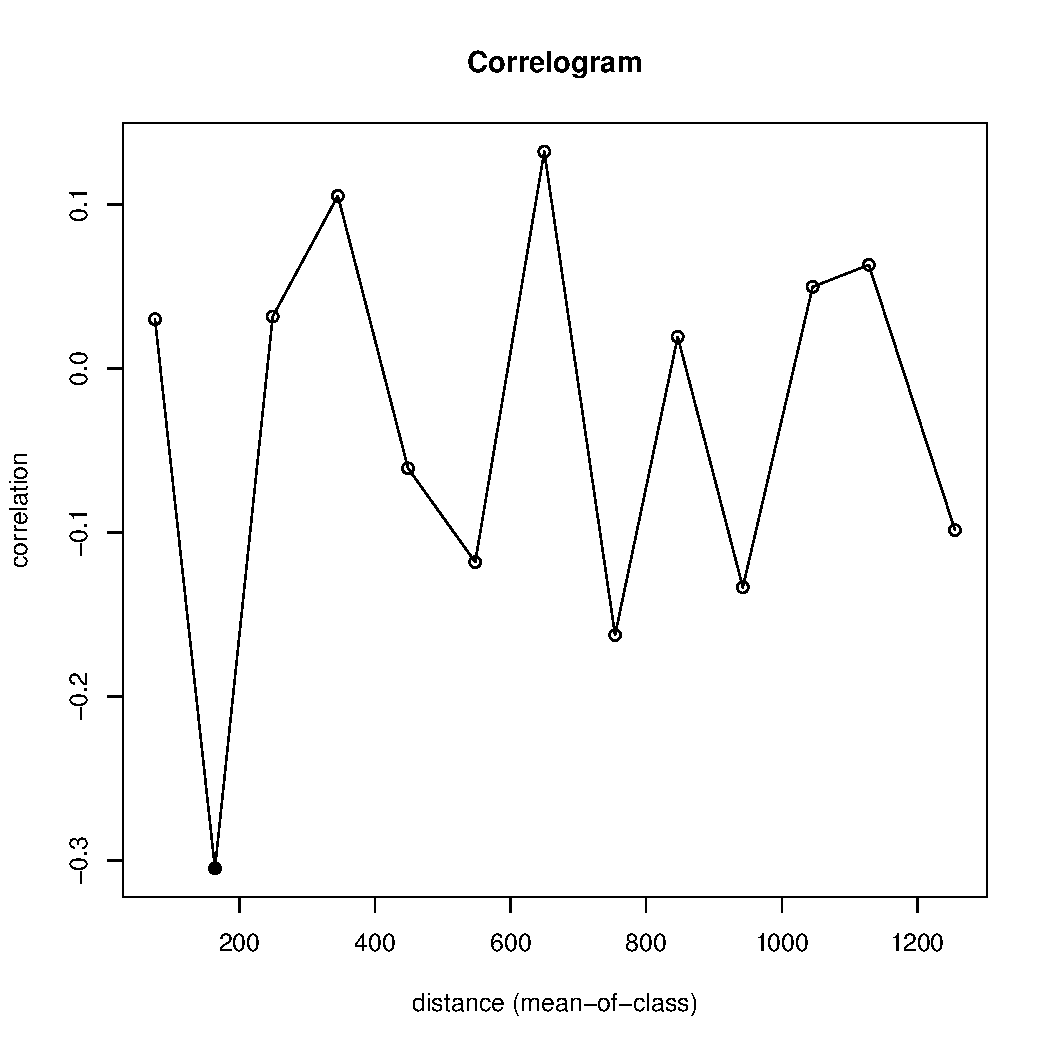
\includegraphics[width=65mm]{../Barenc_Sea/distribution_Moran/Plyazh081_moran_B_Macoma_balthica_.pdf}
	\end{center}
	\end{minipage}

	
	\begin{minipage}[b]{.46\linewidth}
	%Фигурка в первом ряду слева размер отведенный под весь этот объект -- 0.46 от ширины строки
	%Параметр [b] означает, что выравнивание этих министраниц будет по нижнему краю
	\begin{center}
	{\small N~{\it Cerastoderma edule} Квадарт 1, 2008}
		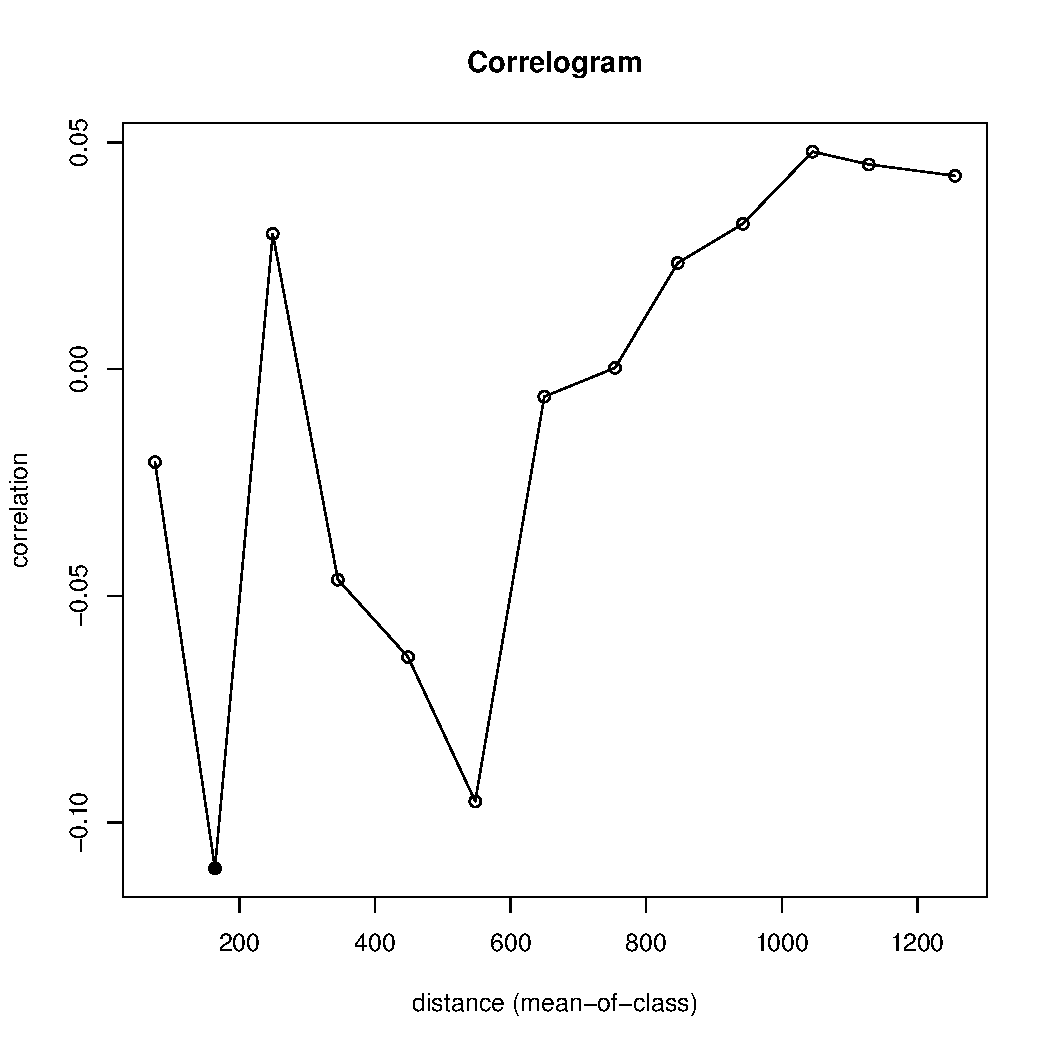
\includegraphics[width=65mm]{../Barenc_Sea/distribution_Moran/Plyazh081_moran_B_Cerastoderma_edule_.pdf}

	\end{center}
	\end{minipage}
	%
	\hfil %Это пружинка отодвигающая рисунки друг от друга
	%
	\begin{minipage}[b]{.46\linewidth}
%Следующий рисунок - первый ряд справа %DUNGEON S_4 \ AB
	\begin{center}
	{\small B~{\it Cerastoderma edule} Квадарт 1, 2008}
		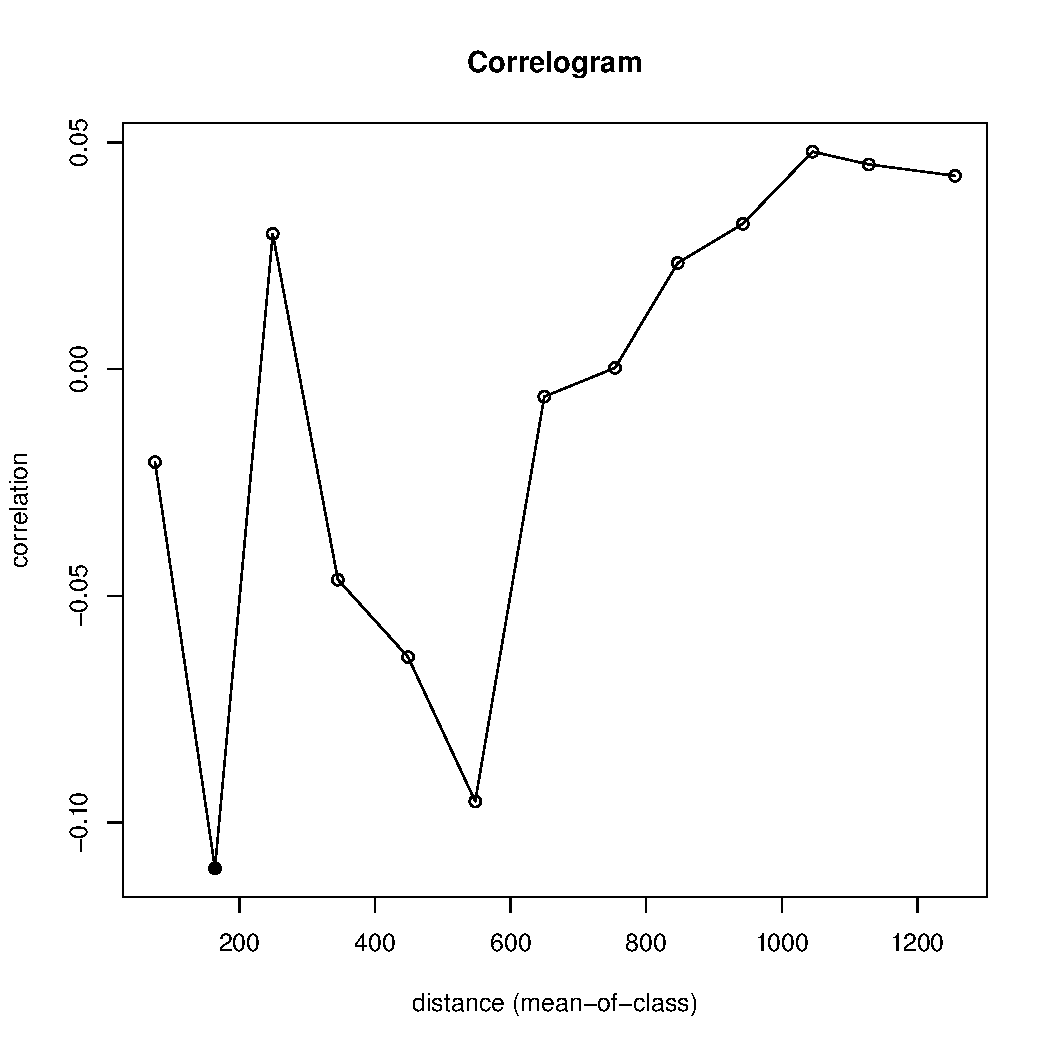
\includegraphics[width=65mm]{../Barenc_Sea/distribution_Moran/Plyazh081_moran_B_Cerastoderma_edule_.pdf}
	\end{center}
	\end{minipage}

	\begin{minipage}[b]{.46\linewidth}
%Фигурка в первом ряду слева размер отведенный под весь этот объект -- 0.46 от ширины строки
%Параметр [b] означает, что выравнивание этих министраниц будет по нижнему краю
	\begin{center}
	{\small N~{\it Gammarus sp.} Квадарт 1, 2008}
		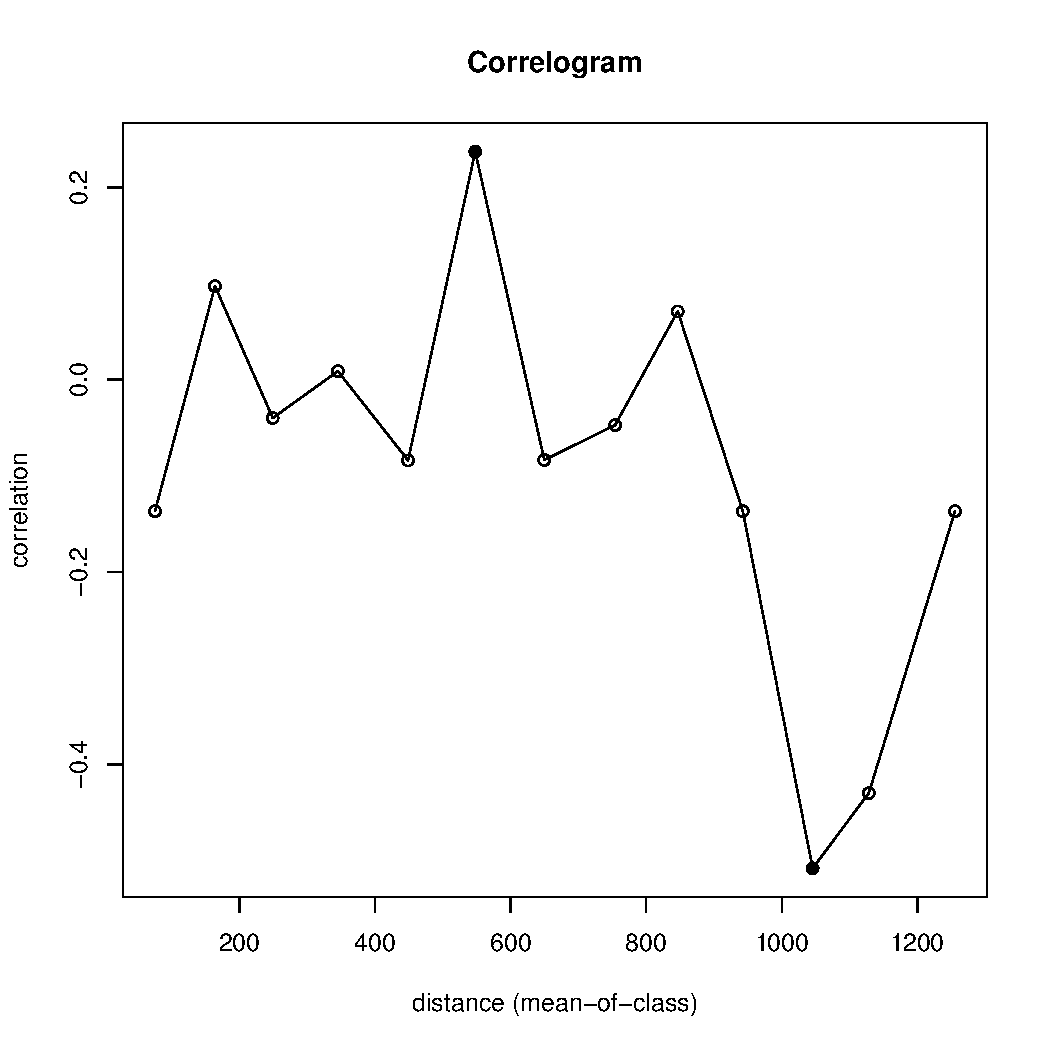
\includegraphics[width=65mm]{../Barenc_Sea/distribution_Moran/Plyazh081_moran_N_Gammarus_sp_.pdf}
	\end{center}
	\end{minipage}
%
	\hfil %Это пружинка отодвигающая рисунки друг от друга
%
	\begin{minipage}[b]{.46\linewidth}
%Следующий рисунок - первый ряд справа %DUNGEON S_4 \ AB
	\begin{center}
	{\small B~{\it Gammarus sp.} Квадарт 1, 2008}
		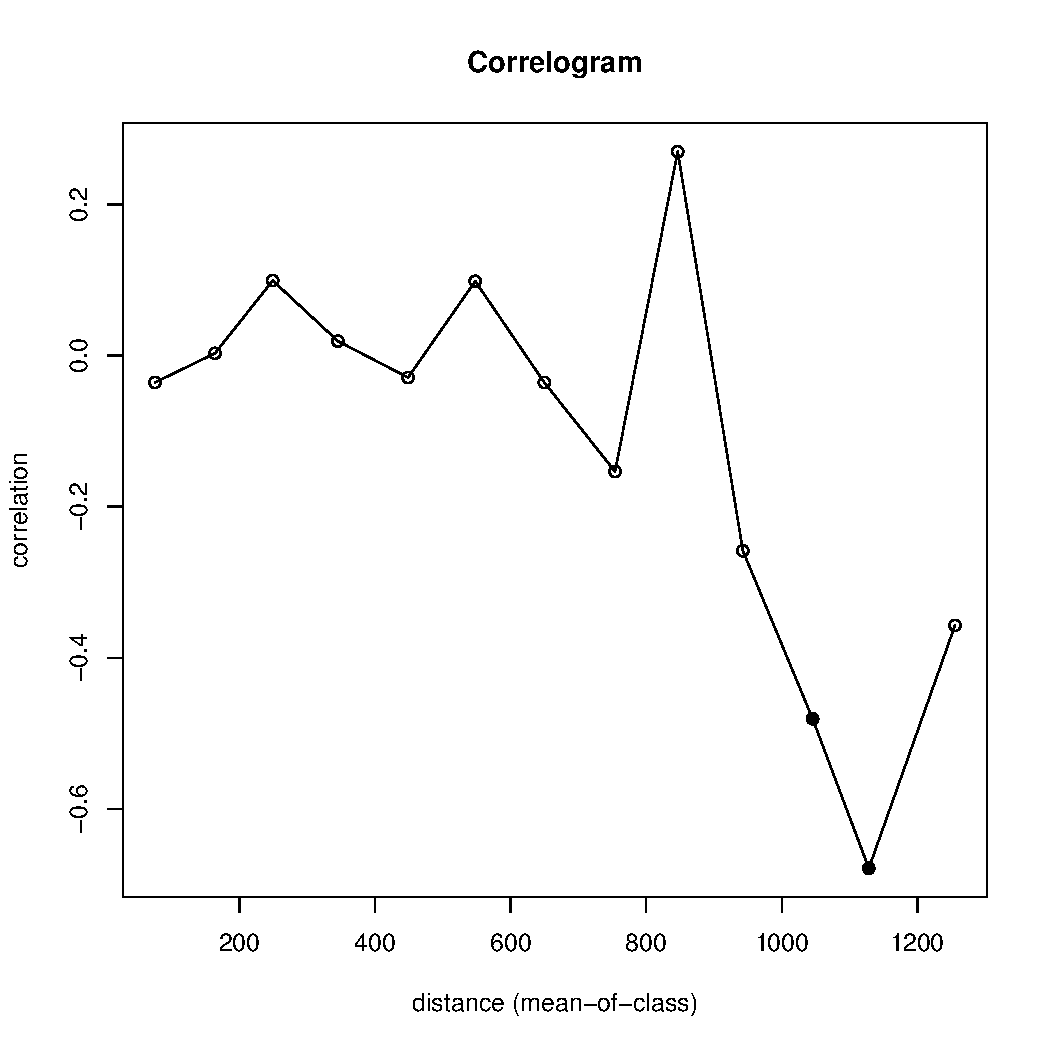
\includegraphics[width=65mm]{../Barenc_Sea/distribution_Moran/Plyazh081_moran_B_Gammarus_sp_.pdf}
	\end{center}
	\end{minipage}


	\begin{minipage}[b]{.46\linewidth}
%Фигурка в первом ряду слева размер отведенный под весь этот объект -- 0.46 от ширины строки
%Параметр [b] означает, что выравнивание этих министраниц будет по нижнему краю
	\begin{center}
	{\small N~{\it Gammarus sp.} 1+2 квадрат, 2008}
		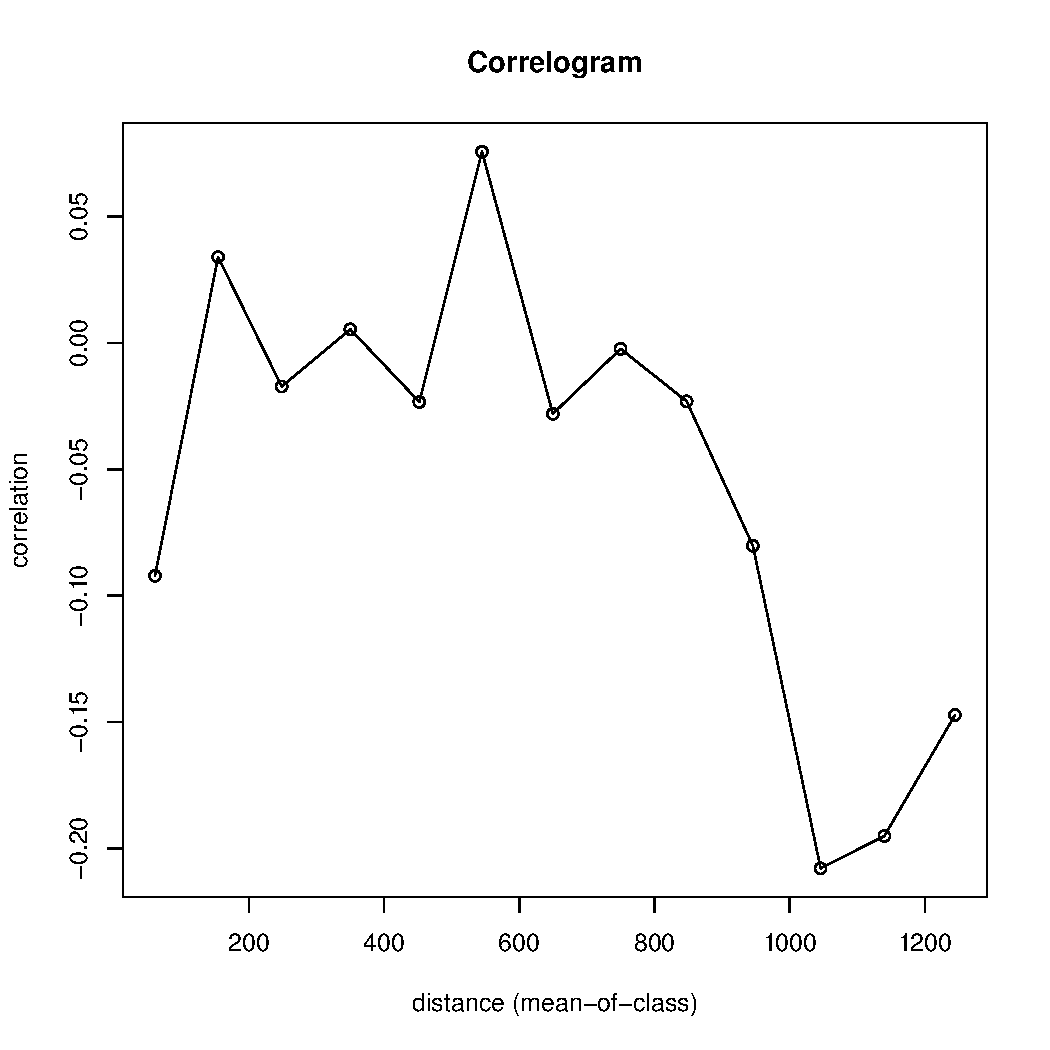
\includegraphics[width=65mm]{../Barenc_Sea/distribution_Moran/Plyazh0812_moran_N_Gammarus_sp_.pdf}
	\end{center}
	\end{minipage}
%
	\hfil %Это пружинка отодвигающая рисунки друг от друга
%
	\begin{minipage}[b]{.46\linewidth}
%Следующий рисунок - первый ряд справа %DUNGEON S_4 \ AB
	\begin{center}
	{\small B~{\it Gammarus sp.} 1+2 квадрат, 2008}
		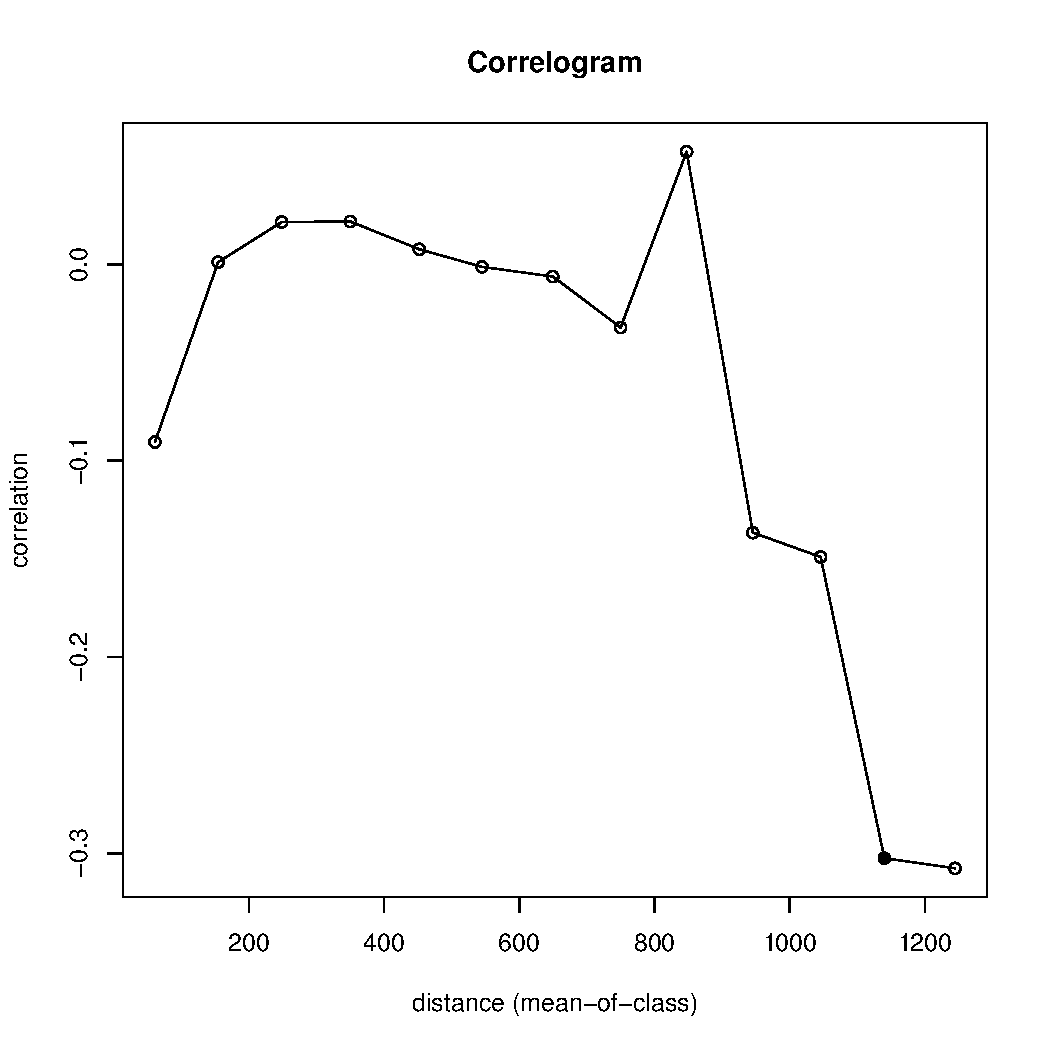
\includegraphics[width=65mm]{../Barenc_Sea/distribution_Moran/Plyazh0812_moran_B_Gammarus_sp_.pdf}
	\end{center}
	\end{minipage}
	\caption{Микрораспределение на литорали Дальнезеленецкой}
	\label{ris:moransI_DZ}
	\end{figure}


{\it P.~caudatus} на литорали Пала-губы формирует агрегации размером $2$ и $4$~м (рис.~\ref{ris:moransI_Pala_Priapulus}). 
Наличие градиента численности, предполагаемого по значениям индекса Морана было подтверждено коэффициентом Кендалла ($\tau = -0,4; p = 0,001$) --- градиент был направлен от ручья.

	\begin{figure}[h]
	\begin{minipage}[b]{.5\linewidth}
	%Фигурка в первом ряду слева размер отведенный под весь этот объект -- 0.46 от ширины строки
	%Параметр [b] означает, что выравнивание этих министраниц будет по нижнему краю
	\begin{center}
	{\small N}
		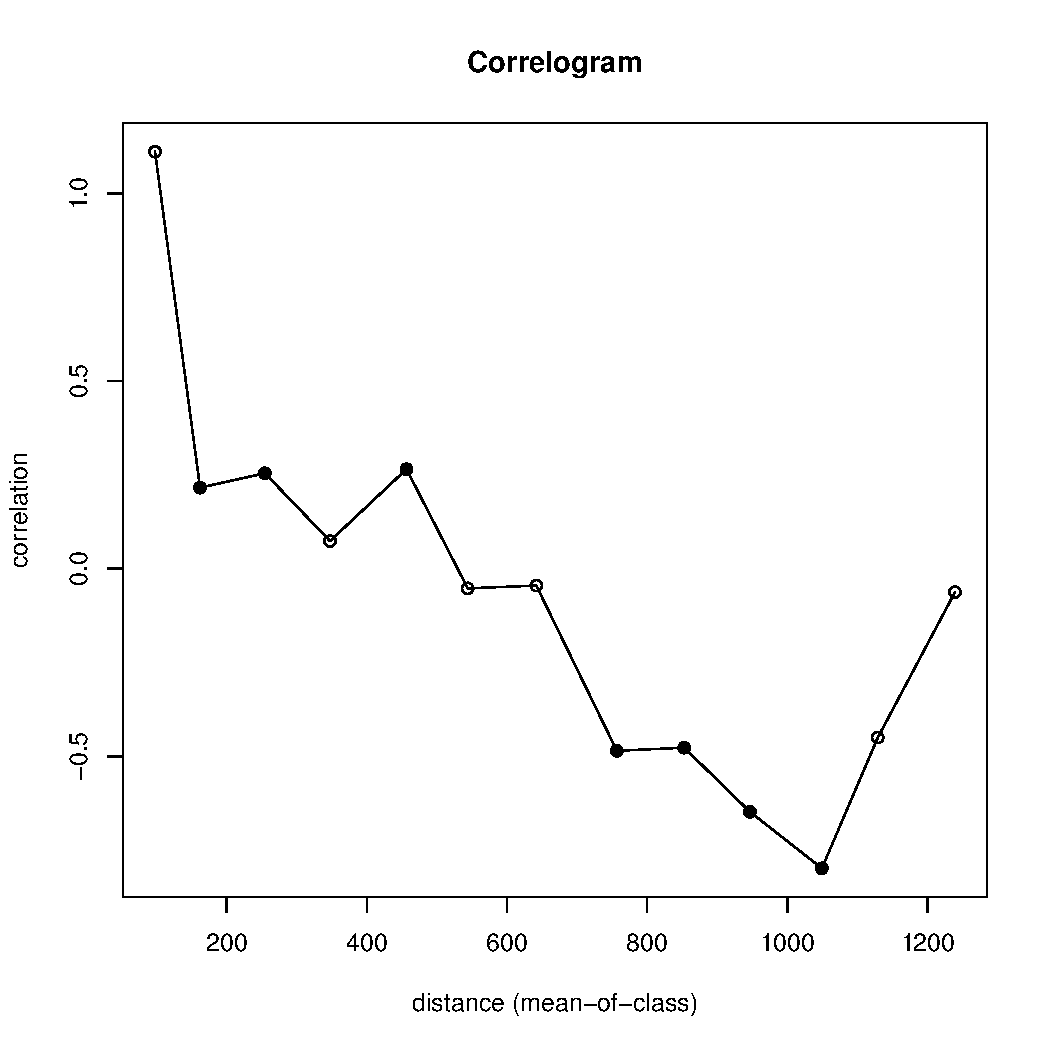
\includegraphics[width=80mm]{../Barenc_Sea/distribution_Moran/Pala_moran_N_Priapulus_caudatus_.pdf}
	\end{center}
	\end{minipage}

	\caption{Микрораспределение {\it Priapulus caudatus} на литорали Пала-губы}
	\label{ris:moransI_Pala_Priapulus}
	\end{figure}



	\subsection{Дальнезеленецкая}
По данным $2007 - 2008$ годов на Дальнем пляже губы Дальнезеленецкая достоверные пятка агрегации были обнаружены для следующих видов: {\it Mya arenaria} ($2007, 2008$ годы), {\it Mytilus edulis} ($2008$), {\it Pseudalibrotus littoralis} ($2008$).

{\it Mya~arenaria} формирует устойчивые скопления размером $1,5 - 2,5$~м (рис.~\ref{ris:moransI_Plyazh_Mya}). 
Кроме того, встречаются пятна размером около $9$~метров.

	\begin{figure}[h]
	\begin{minipage}[b]{.5\linewidth}
	%Фигурка в первом ряду слева размер отведенный под весь этот объект -- 0.46 от ширины строки
	%Параметр [b] означает, что выравнивание этих министраниц будет по нижнему краю
	\begin{center}
	{\small N, $2007$}
		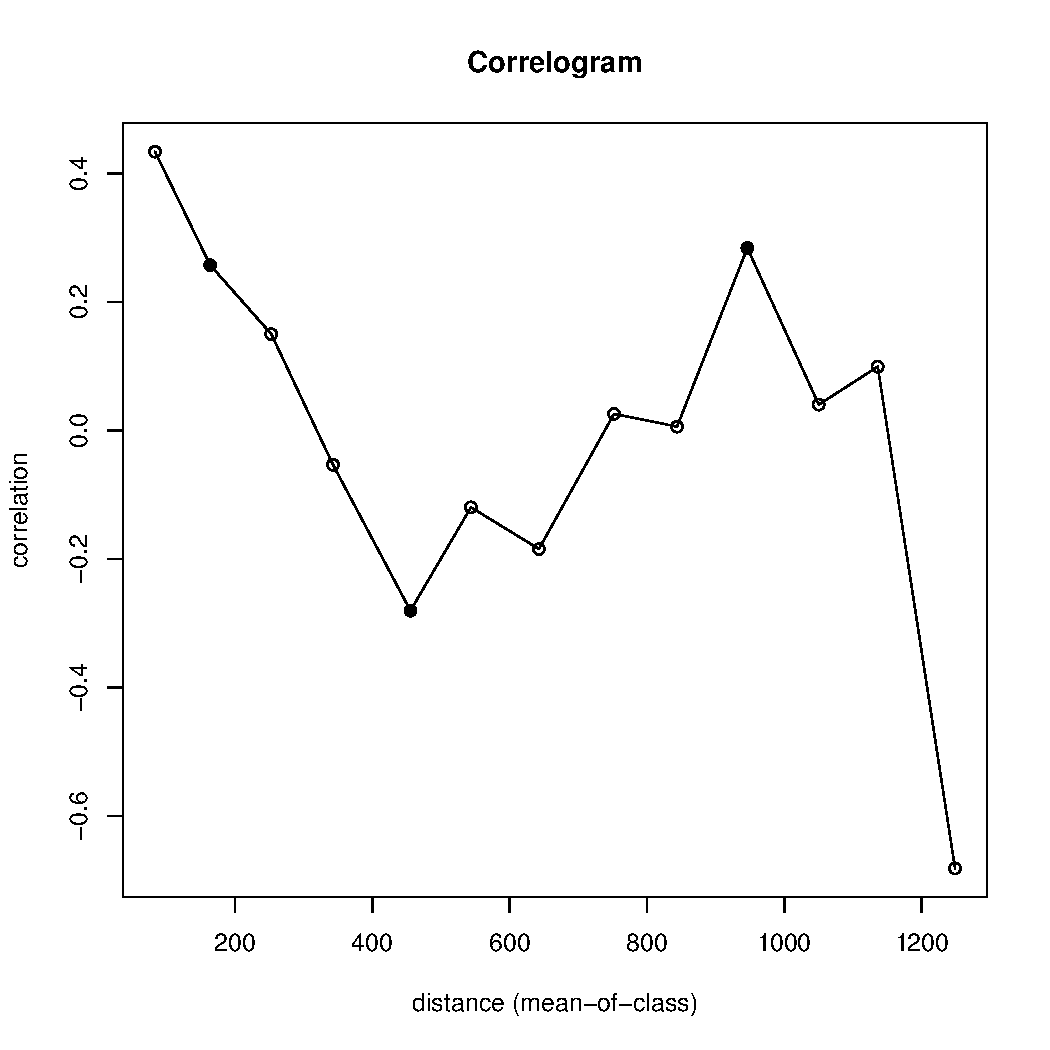
\includegraphics[width=80mm]{../Barenc_Sea/distribution_Moran/Plyazh07_moran_N_Mya_arenaria_.pdf}
	\end{center}
	\end{minipage}
	%
	\hfil %Это пружинка отодвигающая рисунки друг от друга
	%
	\begin{minipage}[b]{.5\linewidth}
	%Фигурка в первом ряду слева размер отведенный под весь этот объект -- 0.46 от ширины строки
	%Параметр [b] означает, что выравнивание этих министраниц будет по нижнему краю
	\begin{center}
	{\small N, $2008$}
		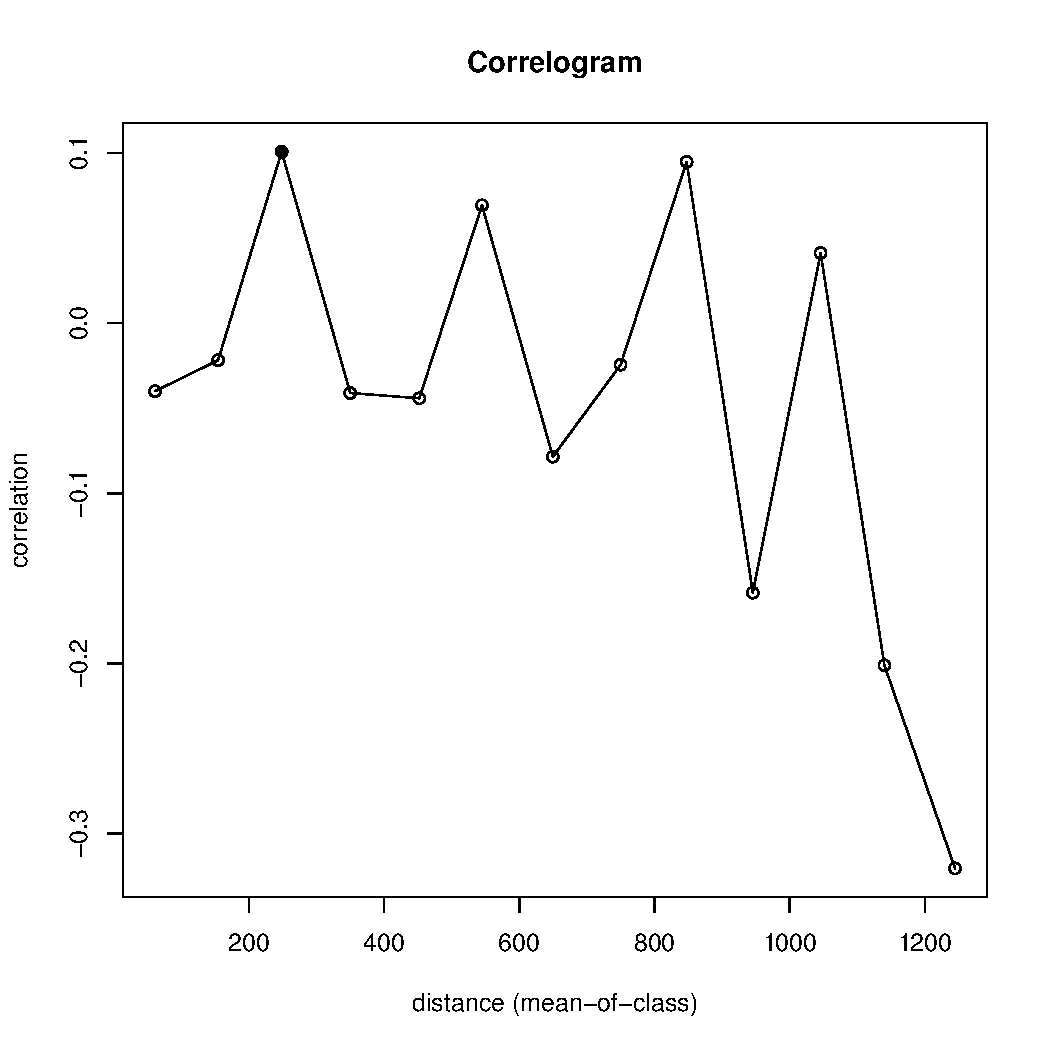
\includegraphics[width=80mm]{../Barenc_Sea/distribution_Moran/Plyazh0812_moran_N_Mya_arenaria_.pdf}
	\end{center}
	\end{minipage}

	\caption{Микрораспределение {\it Mya arenaria} на литорали губы Дальнезеленецкая}
	\label{ris:moransI_Plyazh_Mya}
	\end{figure}

{\it Mytilus~edulis} формирует пятна агрегации размером около $10$~м (рис.~\ref{ris:moransI_Plyazh_Mytilus}). 
Интересно, что для мидий коррелограммы, полученные по данным о численности и о биомассе, не совпадают. 
По данным о биомассе мидий, скопления данных моллюсков размером около $1$ метра на литорали располагаются на расстоянии около $7$ метров.

	\begin{figure}[h]
	\begin{minipage}[b]{.5\linewidth}
	%Фигурка в первом ряду слева размер отведенный под весь этот объект -- 0.46 от ширины строки
	%Параметр [b] означает, что выравнивание этих министраниц будет по нижнему краю
	\begin{center}
	{\small N, $2008$}
		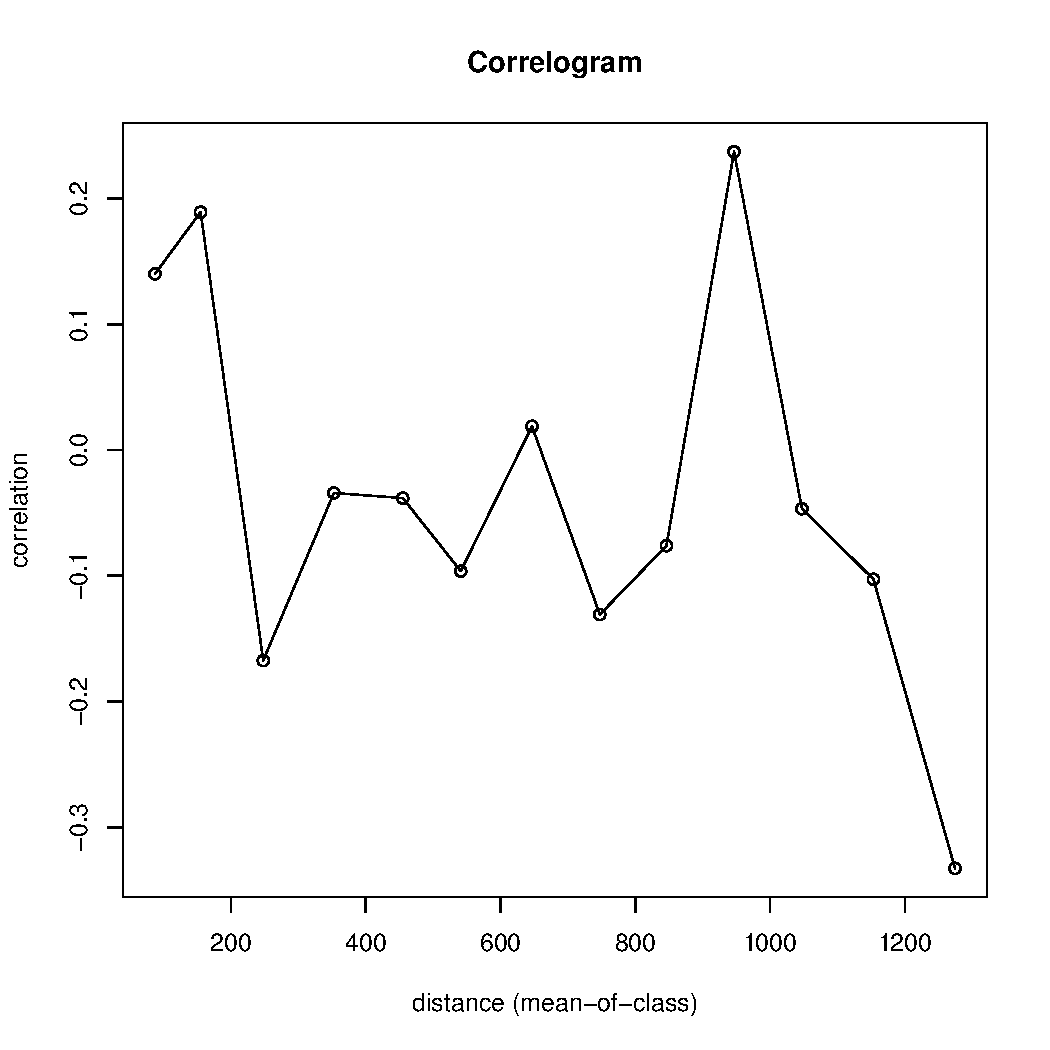
\includegraphics[width=80mm]{../Barenc_Sea/distribution_Moran/Plyazh082_moran_N_Mytilus_edulis_.pdf}
	\end{center}
	\end{minipage}
	%
	\hfil %Это пружинка отодвигающая рисунки друг от друга
	%
	\begin{minipage}[b]{.5\linewidth}
	%Следующий рисунок - первый ряд справа %DUNGEON S_4 \ AB
	\begin{center}
	{\small B, $2008$}
		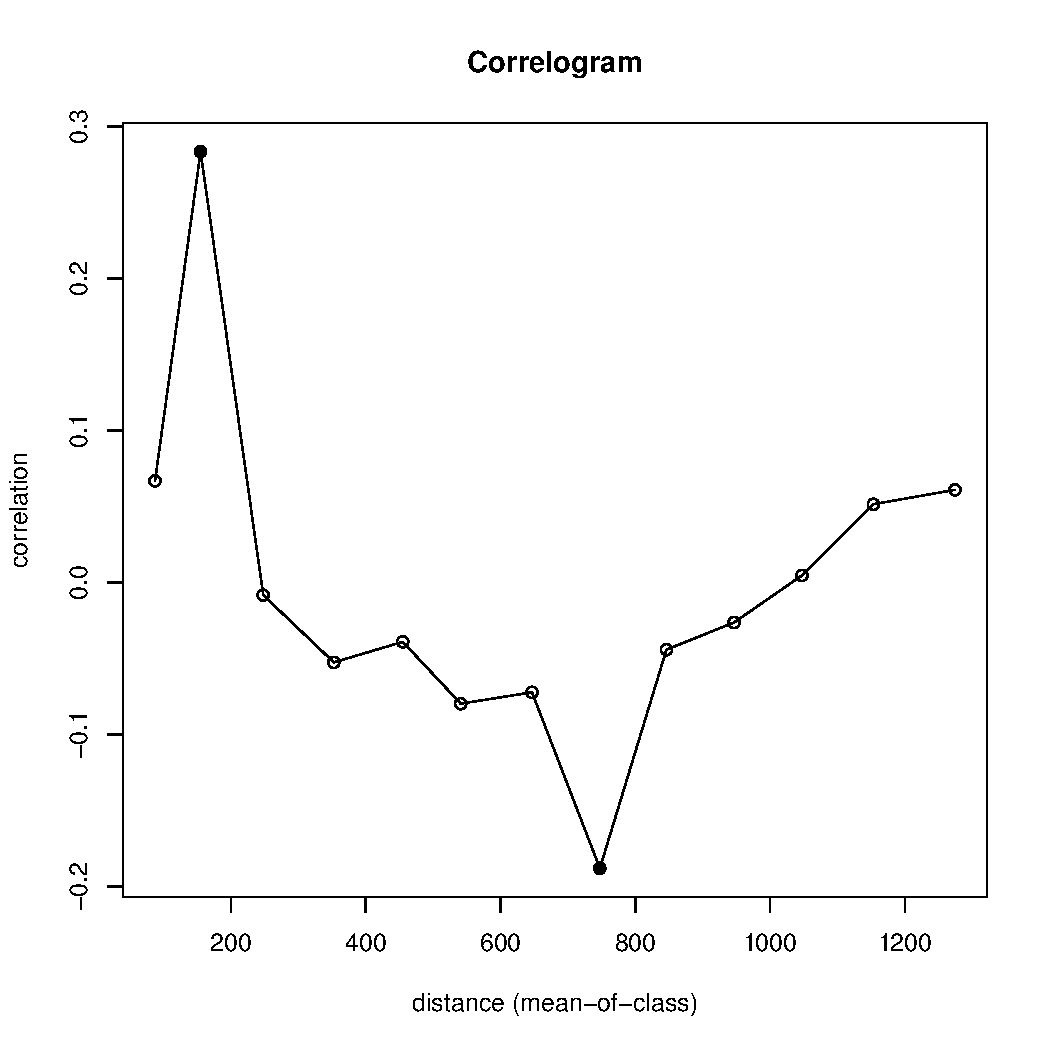
\includegraphics[width=80mm]{../Barenc_Sea/distribution_Moran/Plyazh082_moran_B_Mytilus_edulis_.pdf}
	\end{center}
	\end{minipage}


	\caption{Микрораспределение {\it Mytilus edulis} на литорали губы Дальнезеленецкая}
	\label{ris:moransI_Plyazh_Mytilus}
	\end{figure}

{\it P.~littoralis} формирует скопления размером около $3$ метров (рис.~\ref{ris:moransI_Plyazh_Pseudalibrotus}).

	\begin{figure}[h]
	\begin{minipage}[b]{.5\linewidth}
	%Фигурка в первом ряду слева размер отведенный под весь этот объект -- 0.46 от ширины строки
	%Параметр [b] означает, что выравнивание этих министраниц будет по нижнему краю
	\begin{center}
	{\small N, $2008$}
		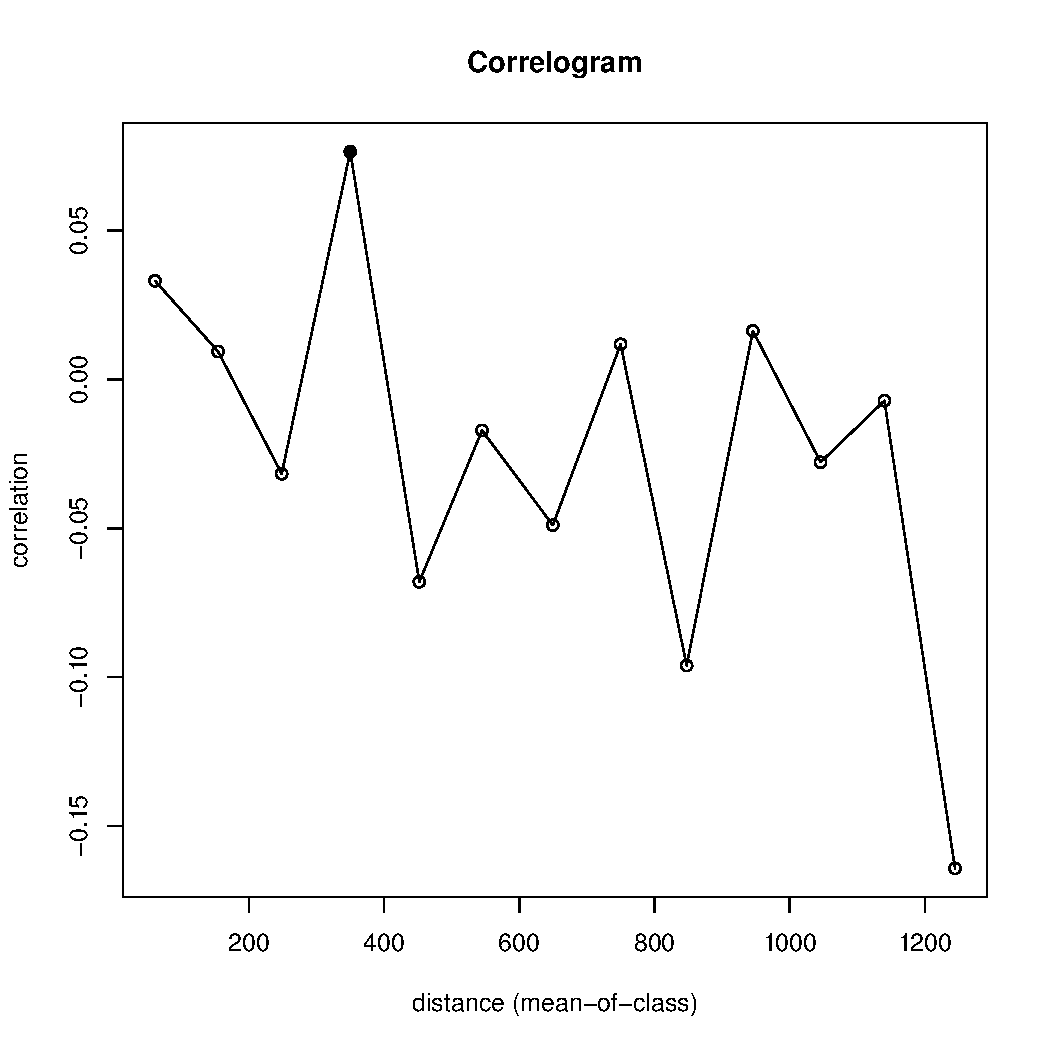
\includegraphics[width=80mm]{../Barenc_Sea/distribution_Moran/Plyazh0812_moran_N_Pseudolibrotus_littoralis_.pdf}
	\end{center}
	\end{minipage}

	\caption{Микрораспределение {\it Pseudalibrotus littoralis} на литорали губы Дальнезеленецкая}
	\label{ris:moransI_Plyazh_Pseudalibrotus}
	\end{figure}


\subsection{Ярнышная}
В губе Ярнышная агрегированное распределение было отмечено только для {\it Mytilus edulis} (рис.~\ref{ris:moransI_Yarnyshnaya_Mytilus}), размер пятен составлял $1 - 5$ метров. 
Наличие серии достоверно отрицательных значений индекса автокорреляции Морана для больших расстояний свидетельствует о наличии либо градиентого изменения численности, либо крупной агрегации с нечеткими краями.
Градиент в направлении к ручью был подствержден в ходе корреляционного анализа методом Кендалла ($\tau = 0,49; p = 3,24 \times 10^{-5}$).

	\begin{figure}[h]
	\begin{minipage}[b]{.5\linewidth}
	%Фигурка в первом ряду слева размер отведенный под весь этот объект -- 0.46 от ширины строки
	%Параметр [b] означает, что выравнивание этих министраниц будет по нижнему краю
	\begin{center}
	{\small N, $2008$}
	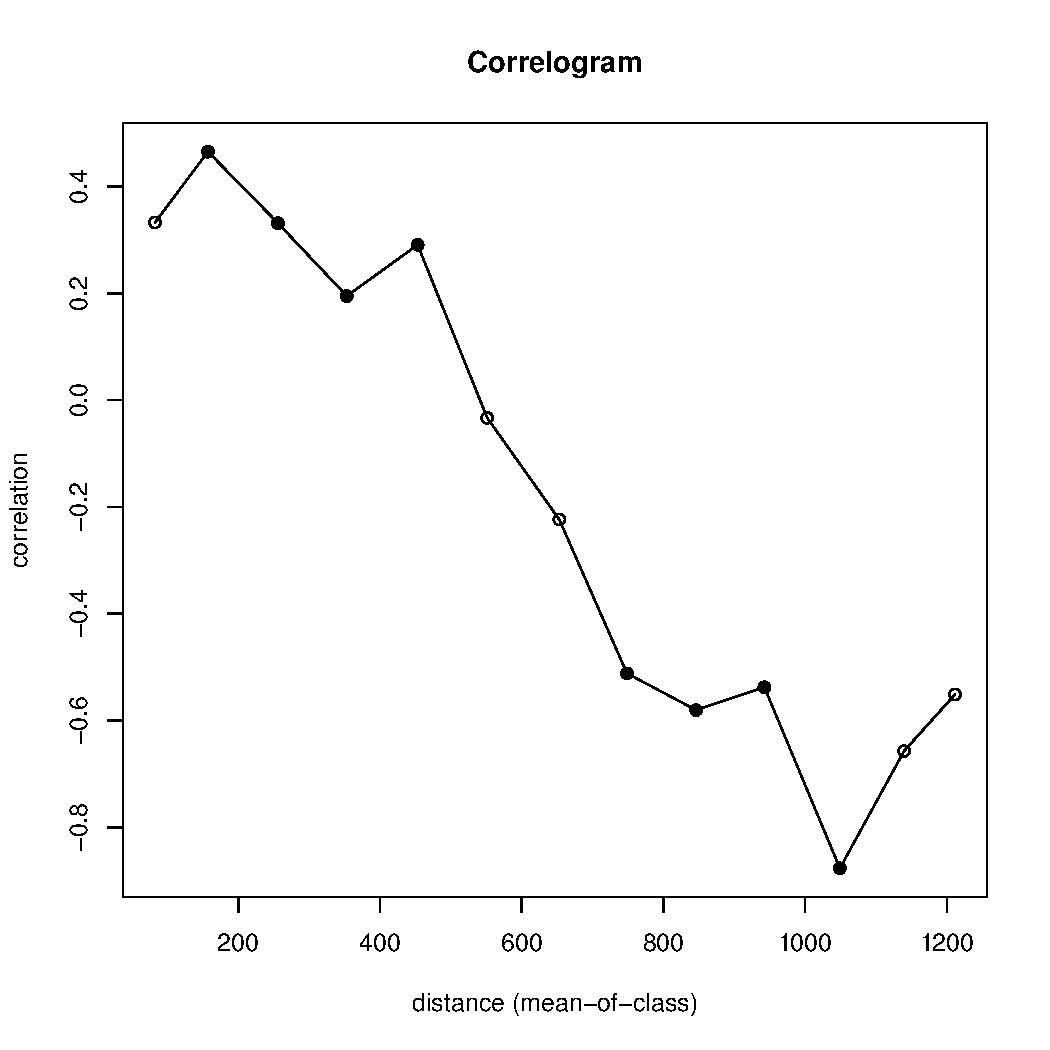
\includegraphics[width=80mm]{../Barenc_Sea/distribution_Moran/Yarnyshnaya07_moran_N_Mytilus_edulis_.pdf}
	\end{center}
	\end{minipage}

	\caption{Микрораспределение {\it Mytilus edulis} на литорали губы Ярнышная}
	\label{ris:moransI_Yarnyshnaya_Mytilus}
	\end{figure}


